% This file was created by tikzplotlib v0.9.8.
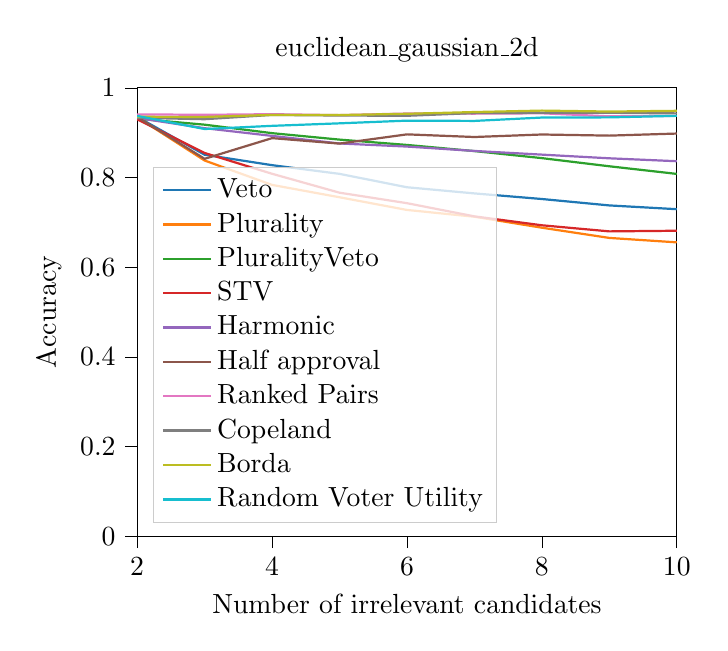
\begin{tikzpicture}

\definecolor{color0}{rgb}{0.12156862745098,0.466666666666667,0.705882352941177}
\definecolor{color1}{rgb}{1,0.498039215686275,0.0549019607843137}
\definecolor{color2}{rgb}{0.172549019607843,0.627450980392157,0.172549019607843}
\definecolor{color3}{rgb}{0.83921568627451,0.152941176470588,0.156862745098039}
\definecolor{color4}{rgb}{0.580392156862745,0.403921568627451,0.741176470588235}
\definecolor{color5}{rgb}{0.549019607843137,0.337254901960784,0.294117647058824}
\definecolor{color6}{rgb}{0.890196078431372,0.466666666666667,0.76078431372549}
\definecolor{color7}{rgb}{0.737254901960784,0.741176470588235,0.133333333333333}
\definecolor{color8}{rgb}{0.0901960784313725,0.745098039215686,0.811764705882353}

\begin{axis}[
legend cell align={left},
legend style={
  fill opacity=0.8,
  draw opacity=1,
  text opacity=1,
  at={(0.03,0.03)},
  anchor=south west,
  draw=white!80!black
},
tick align=outside,
tick pos=left,
title={euclidean\_gaussian\_2d},
x grid style={white!69.0196078431373!black},
xlabel={Number of irrelevant candidates},
xmin=2, xmax=10,
xtick style={color=black},
y grid style={white!69.0196078431373!black},
ylabel={Accuracy},
ymin=0, ymax=1,
ytick style={color=black}
]
\addplot [thick, color0]
table {%
2 0.9354
3 0.8509
4 0.8276
5 0.8082
6 0.7783
7 0.7646
8 0.7521
9 0.7378
10 0.7294
};
\addlegendentry{Veto}
\addplot [thick, color1]
table {%
2 0.9346
3 0.838
4 0.7836
5 0.756
6 0.7277
7 0.7126
8 0.6881
9 0.6653
10 0.6554
};
\addlegendentry{Plurality}
\addplot [thick, color2]
table {%
2 0.9313
3 0.9179
4 0.899
5 0.8846
6 0.8727
7 0.859
8 0.8433
9 0.8251
10 0.8081
};
\addlegendentry{PluralityVeto}
\addplot [thick, color3]
table {%
2 0.9299
3 0.8548
4 0.8084
5 0.7662
6 0.7428
7 0.7134
8 0.6935
9 0.6799
10 0.6813
};
\addlegendentry{STV}
\addplot [thick, color4]
table {%
2 0.9329
3 0.9101
4 0.8929
5 0.876
6 0.8691
7 0.8593
8 0.8511
9 0.8429
10 0.8364
};
\addlegendentry{Harmonic}
\addplot [thick, color5]
table {%
2 0.935
3 0.8418
4 0.8879
5 0.8757
6 0.8963
7 0.8904
8 0.896
9 0.8935
10 0.8981
};
\addlegendentry{Half approval}
\addplot [thick, color6]
table {%
2 0.9409
3 0.9399
4 0.9413
5 0.9392
6 0.9428
7 0.9425
8 0.9433
9 0.9365
10 0.9376
};
\addlegendentry{Ranked Pairs}
\addplot [thick, white!49.8039215686275!black]
table {%
2 0.9333
3 0.9301
4 0.9396
5 0.9383
6 0.9377
7 0.9438
8 0.9443
9 0.9444
10 0.9431
};
\addlegendentry{Copeland}
\addplot [thick, color7]
table {%
2 0.9354
3 0.9352
4 0.9397
5 0.9394
6 0.9422
7 0.9461
8 0.9493
9 0.9472
10 0.9488
};
\addlegendentry{Borda}
\addplot [thick, color8]
table {%
2 0.9375
3 0.9082
4 0.9153
5 0.9209
6 0.9269
7 0.9263
8 0.9338
9 0.9342
10 0.9376
};
\addlegendentry{Random Voter Utility}
\end{axis}

\end{tikzpicture}
